
作为软件开发中的常用工具,CMake可以与各种IDE和源代码编辑器集成。在使用IDE或编辑器的同时,这样的集成对用户来说可能会更方便。本节中,将介绍CMake如何与一些流行的IDE和编辑器的集成。

若希望获得关于如何使用IDE或编辑器的指南,这一节将不会涉及这些内容。本节的主要重点是研究和学习CMake与这些工具的集成。本节假设读者已有使用将要交互的IDE/编辑器的经验。

先从Visual Studio开始吧!

\subsubsubsection{2.4.1\hspace{0.2cm}Visual Studio}

Visual Studio是支持CMake的后来者之一。与其他流行的IDE不同,Visual Studio直到2017年才原生支持CMake。那一年,微软决定采取行动,引入了对处理CMake项目的内置支持,并发布了Visual Studio 2017。从那时起,内置支持CMake就成为了Visual Studio IDE的一个可靠特性。

开始介绍前,请获取一份Visual Studio 2017或更高版本的副本,对于老版本的Visual Studio没有这个特性。我们的例子中,将使用Visual Studio 2022社区版。

\hspace*{\fill} \\ %插入空行
\noindent
\textbf{从头开始创建一个CMake项目}

Visual Studio项目创建特性是基于项目模板的。在VS2017及以上版本中,项目模板也包含一个CMake项目模板。我们将学习如何使用这个模板来创建新的CMake项目。

要用Visual Studio创建一个新的CMake项目,请单击欢迎页面上的create a new project按钮。或者,可以通过在主IDE窗口中单击File | New | Project来访问,或者使用Ctrl + Shift + N (New Project)快捷键。VS2022的欢迎界面是这样的:

\begin{center}
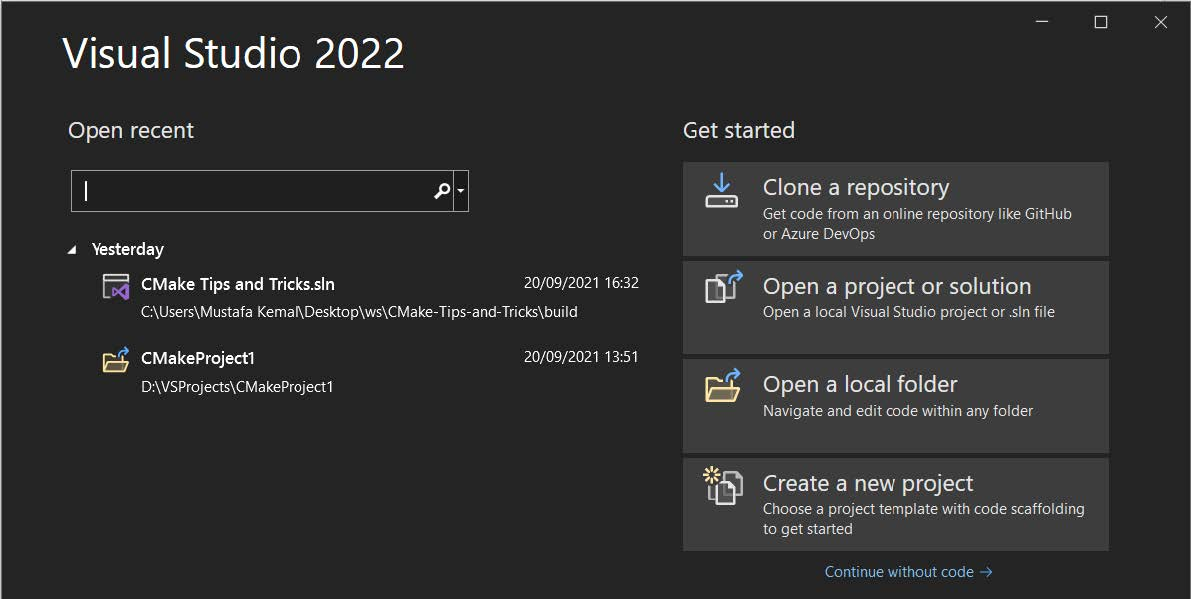
\includegraphics[width=0.8\textwidth]{content/1/chapter2/images/35.jpg}\\
图2.35 Visual Studio 2022欢迎界面
\end{center}

在“创建新项目”窗口上,双击项目模板列表中的CMake project。可以使用位于列表顶部的搜索栏来筛选项目模板:

\begin{center}
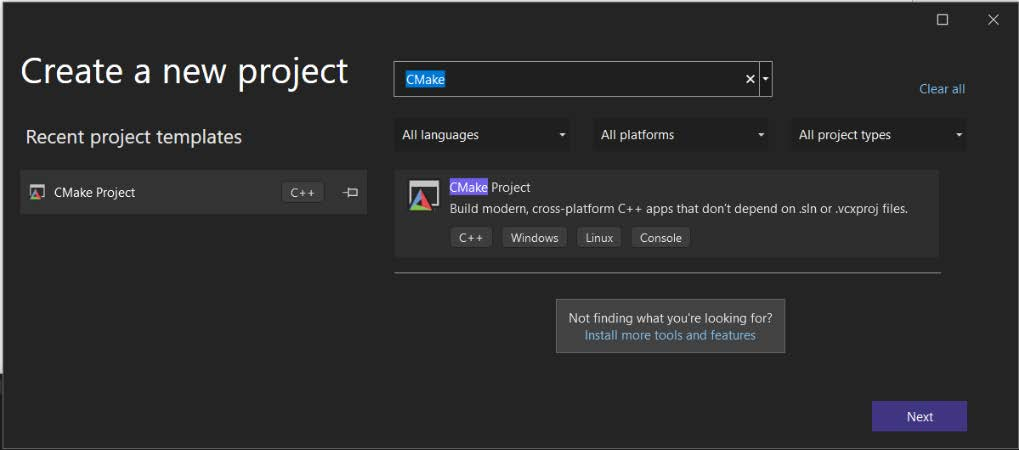
\includegraphics[width=0.8\textwidth]{content/1/chapter2/images/36.jpg}\\
图2.36 - Visual Studio 2022创建新项目界面
\end{center}

单击Next之后,将出现项目配置窗口。可以给CMake项目起一个名字,并选择将新项目放在哪里。在我们的示例中,将使用默认项目名称CMakeProject1。

\begin{center}
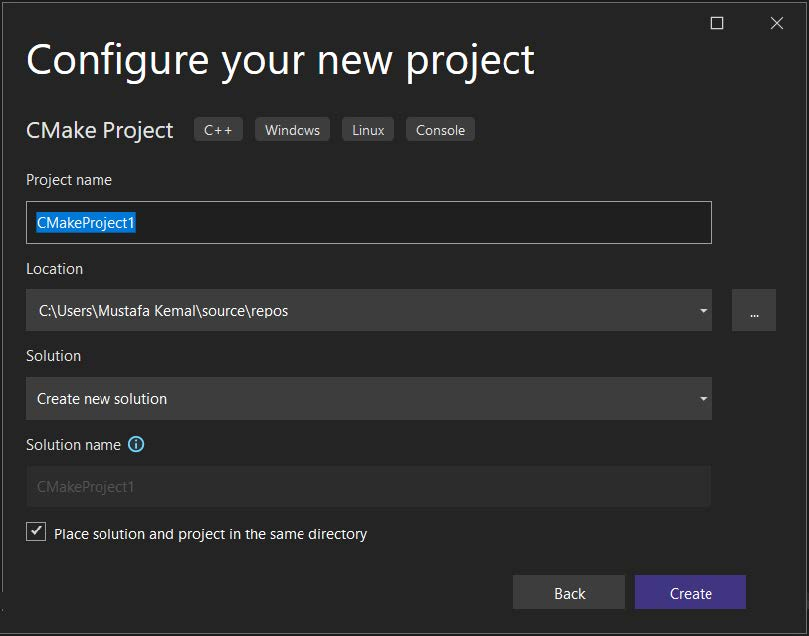
\includegraphics[width=0.8\textwidth]{content/1/chapter2/images/37.jpg}\\
图2.37  Visual Studio 2022新项目配置界面
\end{center}

填写详细信息后,单击Create创建新的CMake项目。生成的项目将包含一个顶级的CMakeLists.txt文件,一个C++源文件,和一个C++头文件,以所选的项目名称命名。新建的项目布局如下图所示:

\begin{center}
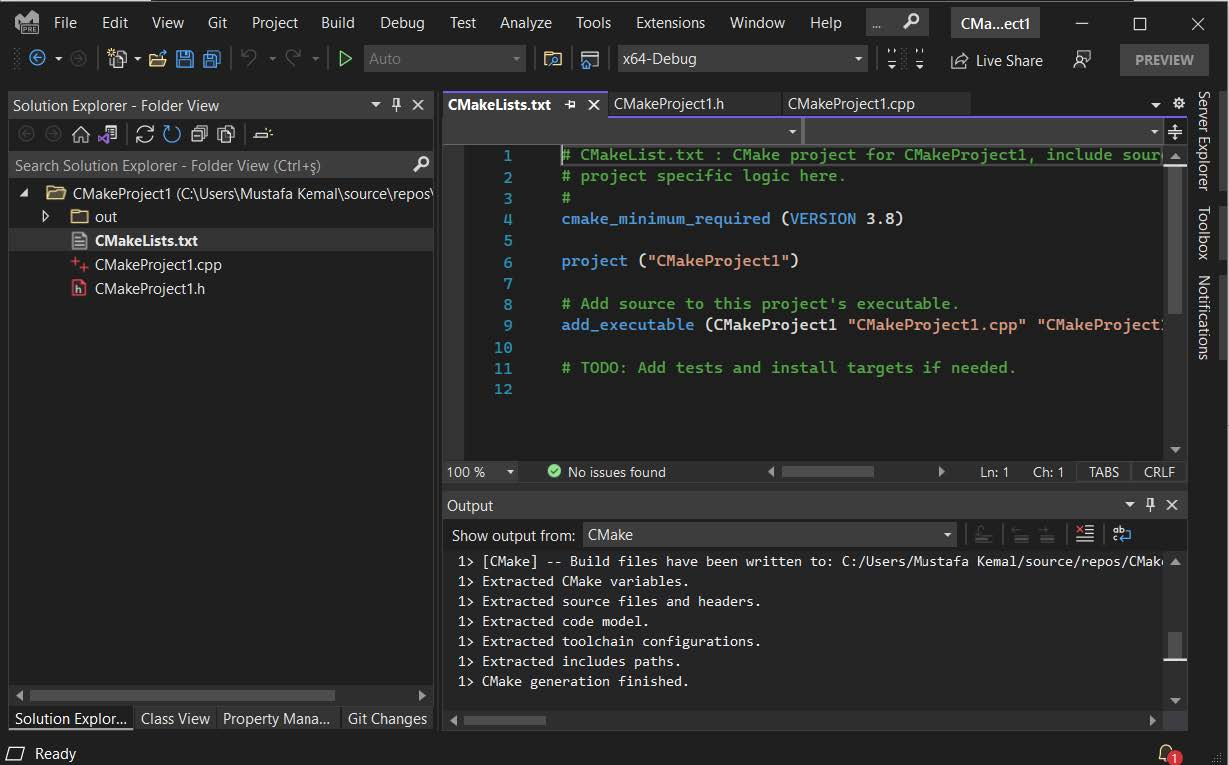
\includegraphics[width=0.8\textwidth]{content/1/chapter2/images/38.jpg}\\
图2.38 用Visual Studio创建的新的CMake项目
\end{center}

\hspace*{\fill} \\ %插入空行
\noindent
\textbf{打开已有的CMake项目}

打开现有的CMake项目,\texttt{File | Open | CMake...}并选择待打开项目的顶层CMakeLists.txt文件。下图显示了“打开”菜单的样子:

\begin{center}
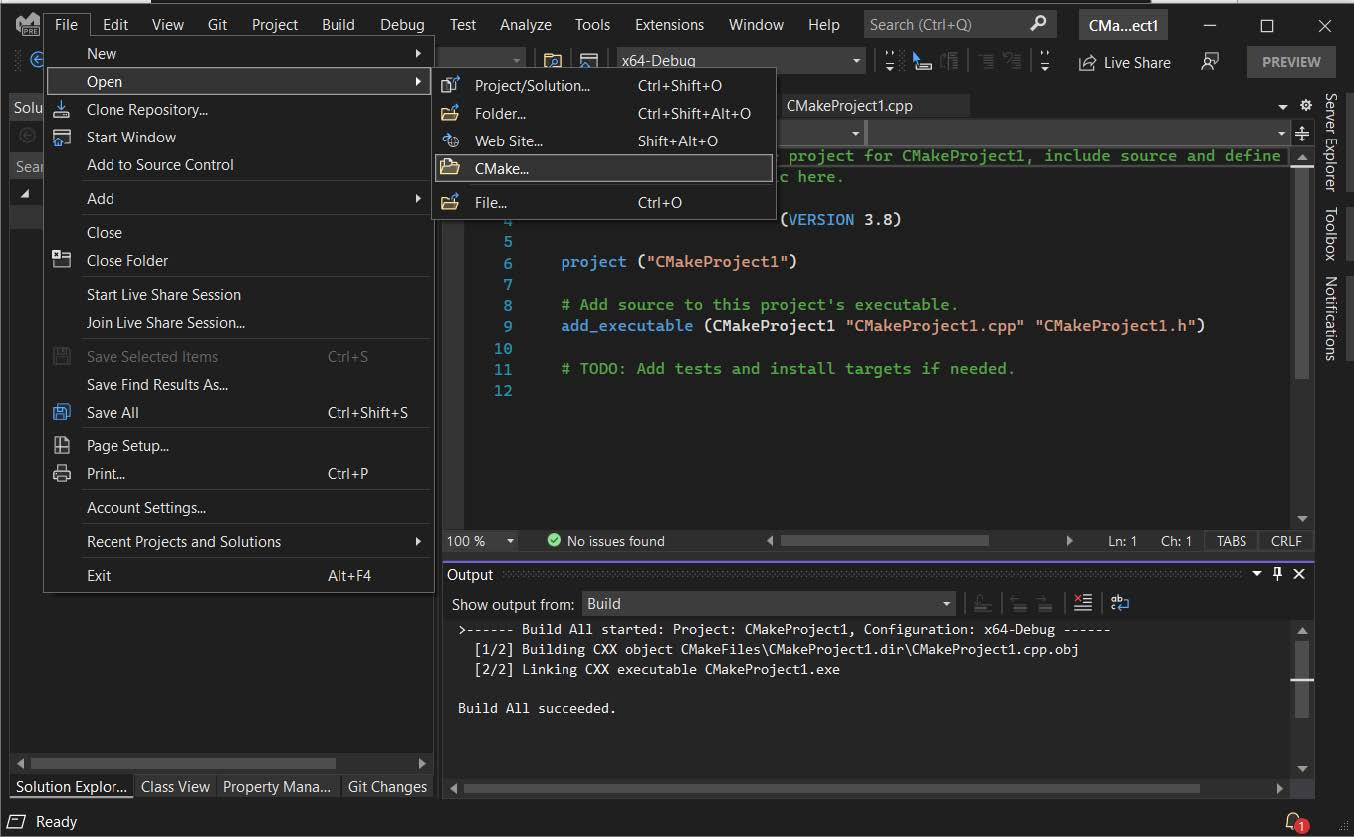
\includegraphics[width=0.8\textwidth]{content/1/chapter2/images/39.jpg}\\
图2.39 CMake项目打开菜单
\end{center}

接下来,让看看如何配置和构建CMake项目。

\hspace*{\fill} \\ %插入空行
\noindent
\textbf{配置和构建CMake项目}

要在Visual Studio中构建CMake项目,请先转到Project | Configure。这将调用CMake配置步骤并生成所需的构建系统文件。配置完成后,单击Build | Build All以生成项目。也可以通过使用F7快捷键来触发Build All。

注意,当保存CMakeLists.txt文件时,Visual Studio将自动重新配置,该文件是项目的一部分。

\hspace*{\fill} \\ %插入空行
\noindent
\textbf{使用CMake目标执行通用操作}

Visual Studio使用启动目标的概念来执行目标所需的操作,比如构建、调试和启动。要将CMake目标设置为启动目标,请使用工具栏上的“选择启动目标”下拉框。Visual Studio将自动在配置中使用CMake目标填充这个下拉框。

\begin{center}
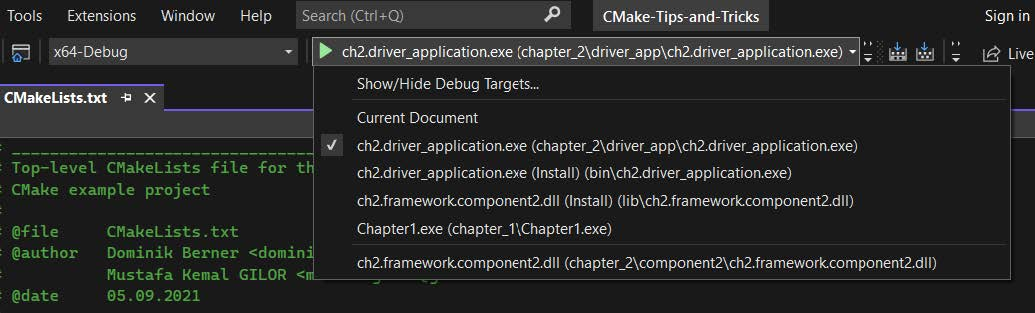
\includegraphics[width=0.8\textwidth]{content/1/chapter2/images/40.jpg}\\
图2.40 启动目标的下拉菜单
\end{center}

设置启动目标后,可以使用诸如调试、构建或启动等操作:

\begin{itemize}
\item 
要调试,首先单击“Debug | Startup Target”,然后单击“Debug | Start Debugging”或使用F5快捷键。

\item 
要在不调试的情况下启动,单击“ Start without debug”或使用Ctrl + F5快捷键。

\item 
要构建,单击Build,或单击Build | Build <target>,或使用Ctrl + B键盘快捷键。

\item
按钮位置如下图所示:

\begin{center}
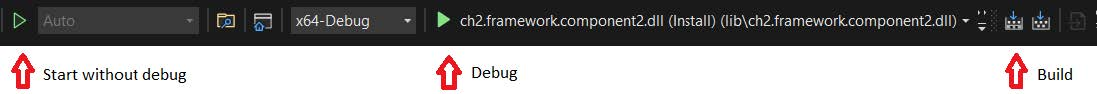
\includegraphics[width=0.8\textwidth]{content/1/chapter2/images/41.jpg}\\
图2.41 工具栏按钮的位置
\end{center}
\end{itemize}

本节中,已经介绍了Visual Studio CMake集成的基础知识。下一节中,将继续了解另一个微软产品,Visual Studio Code。

\subsubsubsection{2.4.2\hspace{0.2cm}Visual Studio Code}

Visual Studio Code (VSCode)是微软开发的一款开源代码编辑器。它不是一个IDE,但可以很强大,并通过扩展具有类似IDE的特性。扩展市场有各种各样的附加内容,从主题到语言服务器。可以找到几乎任何东西的扩展,这使VSCode既强大,喜欢广泛的观众,VSCode也有一个官方的CMake扩展。这个扩展最初是由Colby Pike开发的(也称为vector-of-bool),但现在由微软官方维护。

本节中,将学习如何安装扩展并使用它执行基本的CMake任务。

在继续之前,VSCode必须已经安装在您的环境中。若还没装,请访问\url{https://code.visualstudio.com/learn/get-started/basics}了解下载和安装的详细信息。

此外,我们将经常访问命令面板。强烈建议经常使用来熟悉它,而命令面板是什么?下面是截图:

\begin{center}
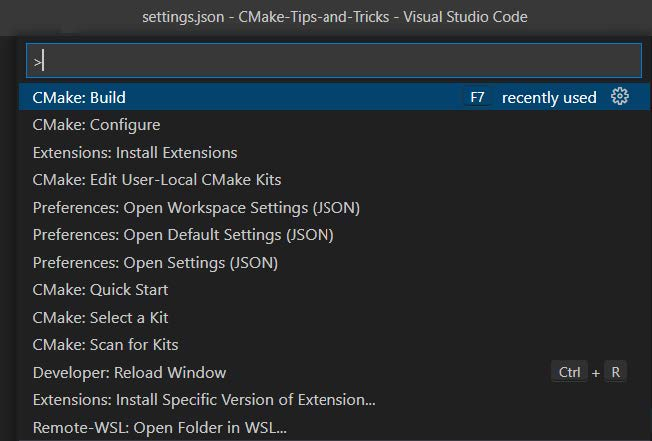
\includegraphics[width=0.6\textwidth]{content/1/chapter2/images/42.jpg}\\
图2.42 VSCode命令面板
\end{center}

说实话,我直到现在才知道它有名字。访问命令面板的快捷键是F1和Ctrl + Shift + p。命令面板是VSCode的面包和黄油,加快了VSCode的工作流程。

\hspace*{\fill} \\ %插入空行
\noindent
\textbf{安装扩展}

安装扩展是非常直接和简单的。要使用CLI安装它,调用以下命令(如果使用的是Insiders版本,则用code-insiders替换code):

\begin{tcblisting}{commandshell={}}
code --install-extension ms-vscode.cmake-tools
\end{tcblisting}

也可以在VSCode GUI中做同样的事情。打开VSCode,单击左侧导航窗格上的Extensions导航到Extensions页面。或者,您可以使用Ctrl + Shift + X快捷键。在扩展搜索框中键入CMake工具,从微软选择CMake工具。注意不要将它与CMake扩展混淆,然后按下安装按钮来安装。

\begin{center}
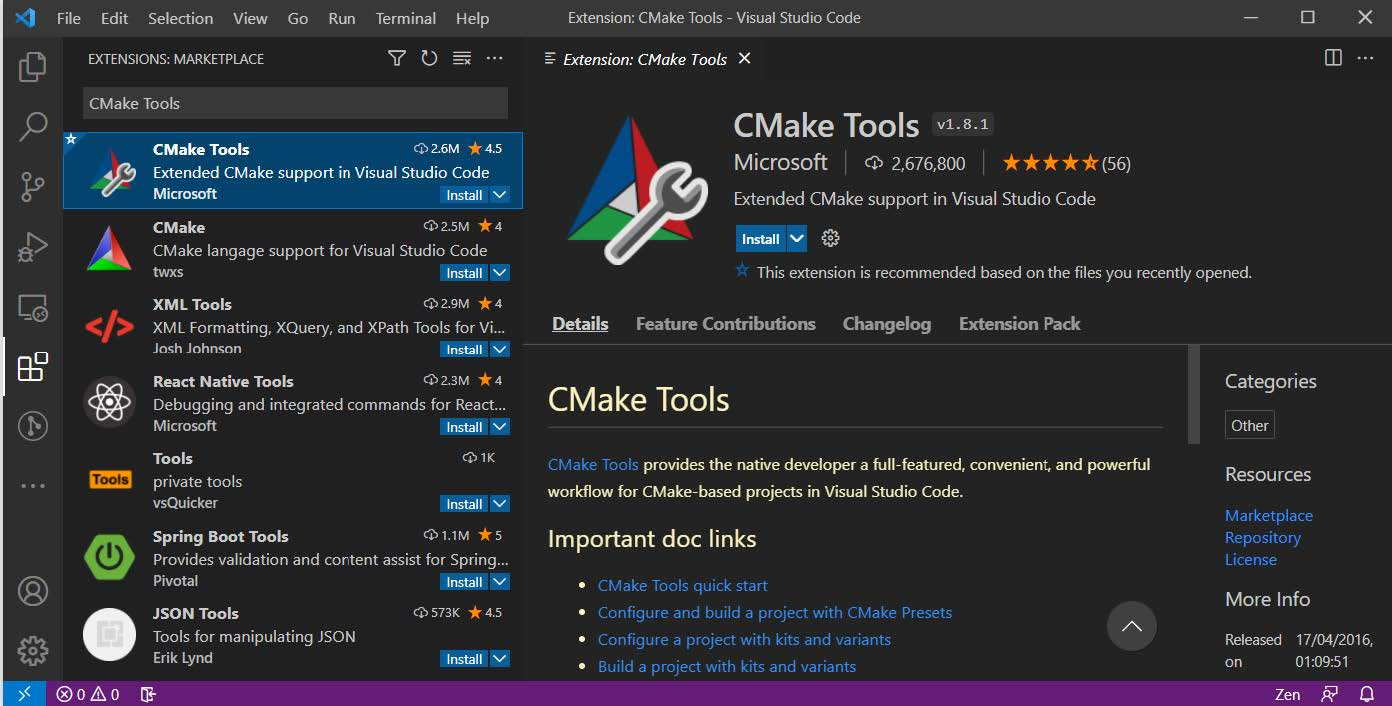
\includegraphics[width=0.8\textwidth]{content/1/chapter2/images/43.jpg}\\
图2.43  VSCode扩展市场
\end{center}

安装完成后,扩展就可以使用了。

\hspace*{\fill} \\ %插入空行
\noindent
\textbf{快速启动项目}

VSCode CMake工具扩展提供了一个快速启动选项,可以引导一个CMake项目,使用示例C++代码。要使用它,首先使用File | Open Folder…打开目标文件夹,然后按F1,并键入\texttt{cmake quick start}。选择“CMake: Quick Start”,按“Enter”键。

\begin{center}
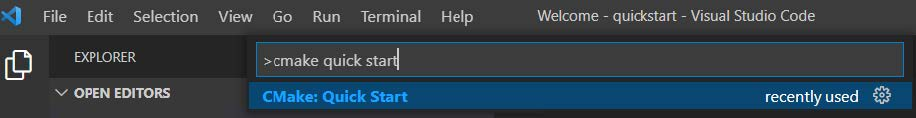
\includegraphics[width=0.8\textwidth]{content/1/chapter2/images/44.jpg}\\
图2.44 命令面板——定位CMake:快速入门
\end{center}

首先,扩展会询问使用哪个套件。选择适合新项目的选项。工具包将在处理工具包一节中会进一步讨论。

选择工具包之后,系统会要求输入项目名称,这将是顶层CMake项目的名称。

最后,将显示选择一个示例应用程序。选择中,将会要求创建一个可执行的应用程序项目或一个库项目。选择其中之一,然后创建CMake项目,CMakeLists.txt和main.cpp文件将自动生成。

\hspace*{\fill} \\ %插入空行
\noindent
\textbf{打开现有的项目}

VSCode中打开CMake项目没什么特别。打开包含项目顶层CMakeLists.txt文件的文件夹,CMake工具扩展将自动识别该文件夹为CMake项目,所有CMake相关的命令将在VSCode命令面板上可用。

\hspace*{\fill} \\ %插入空行
\noindent
\textbf{配置、构建和清理项目}

要配置CMake项目,从命令面板中选择CMake: Configure菜单项。要构建项目,通过从命令面板中选择CMake: Set build target菜单项来选择一个构建目标,可以选择在调用构建时构建的内容。最后,选择CMake: Build来构建选定的构建目标。要生成一个特定的目标而不将其设置为生成目标,请使用CMake: build target菜单项。

要清理构建工件,使用CMake:Clean命令面板项。这将运行CMake的clean目标并删除所有构建工件。

\hspace*{\fill} \\ %插入空行
\noindent
\textbf{调试目标}

要调试一个目标,从命令面板中选择CMake: Set debug target菜单项来选择一个调试目标。会看到列出的可调试目标。

\begin{center}
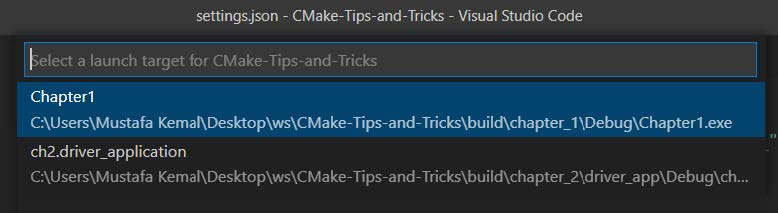
\includegraphics[width=0.8\textwidth]{content/1/chapter2/images/45.jpg}\\
图2.45 选择调试目标
\end{center}

选择目标并从命令面板中选择CMake: Debug (Ctrl + F5),所选目标将在调试器下启动。

若想在没有调试器的情况下运行选定的目标,选择CMake: run without Debugging (Shift + F5)。

\begin{center}
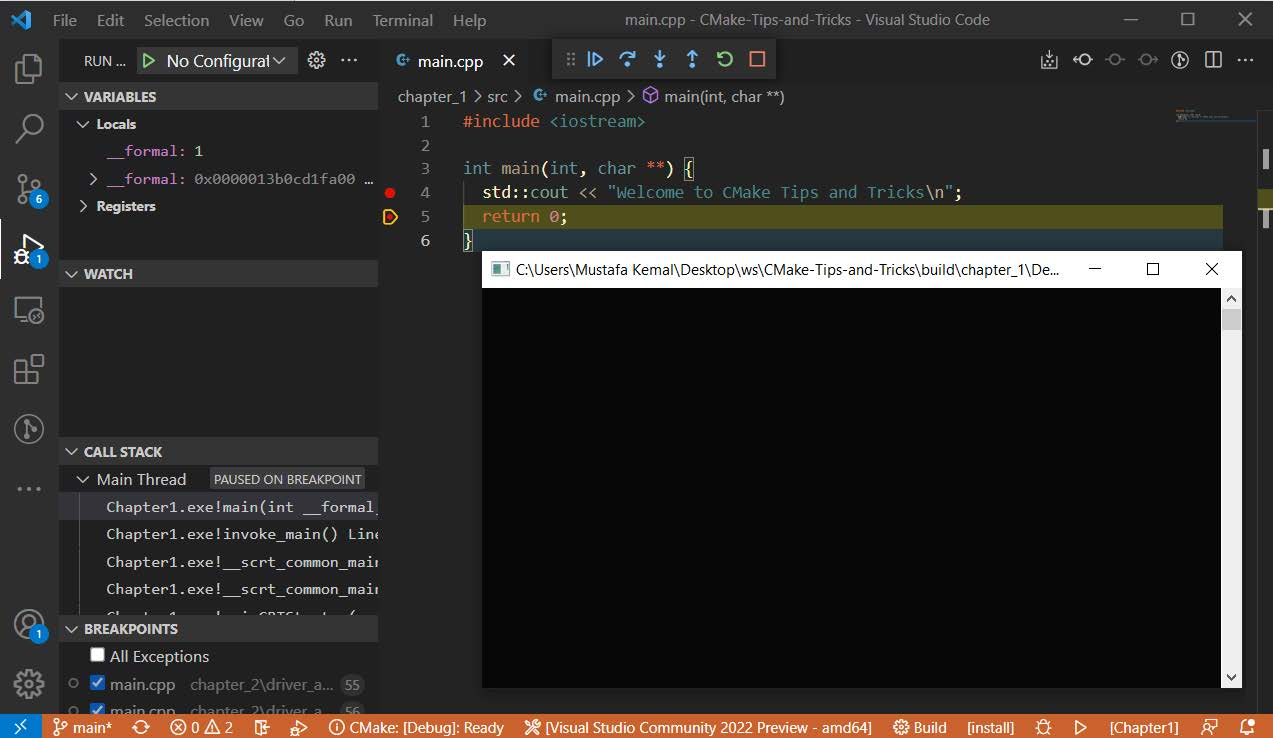
\includegraphics[width=0.8\textwidth]{content/1/chapter2/images/46.jpg}\\
图2.46 正在调试可执行的Chapter1目标
\end{center}

下一节中,将研究如何为已调试的目标提供参数。

\hspace*{\fill} \\ %插入空行
\noindent
\textbf{向调试的目标传递参数}

试图调试的目标可能需要命令行参数。要将命令行参数传递给调试目标,请打开VSCode的settings.json文件,并添加以下行:

\begin{lstlisting}[style=styleCMake]
"cmake.debugConfig": {
		"args": [
		"<argument1>",
		"<argument2>"
		]
	}
\end{lstlisting}

JSON中的args数组中,可以放置目标所需的任意数量的参数。这些参数将无条件地传递给所有未来的调试目标。若希望对参数进行更细粒度的控制,最好定义一个launch.json文件。

\hspace*{\fill} \\ %插入空行
\noindent
\textbf{处理套件}

CMake工具扩展中的套件代表了可用于构建项目的工具组合,套件这个术语几乎就是工具链的同义词。工具包使在多编译器环境中工作变得更容易,允许用户选择使用哪一个编译器。工具包可以通过扩展自动发现、从工具链文件读取或由用户手动定义。

要查看项目可用的套件,选择CMake:从命令面板中选择套件菜单项(F1或Ctrl+Shift+P)。

\begin{center}
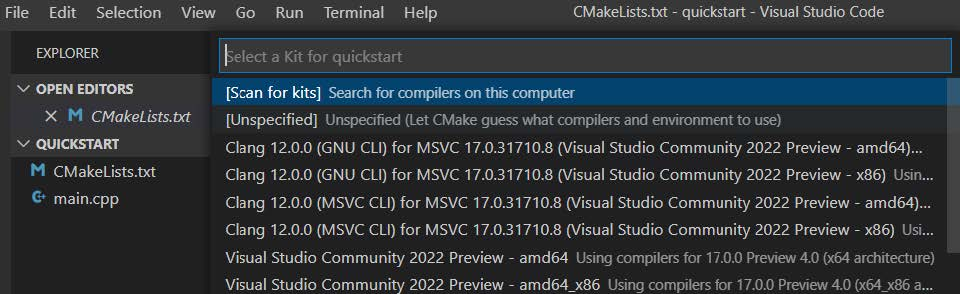
\includegraphics[width=0.8\textwidth]{content/1/chapter2/images/47.jpg}\\
图2.47 套件选择列表
\end{center}

选择的工具包将用于配置CMake项目,从而工具包中定义的工具将用于编译项目。套件选择将自动触发CMake配置。

默认情况下,扩展自动扫描套件。因此,工具链会作为选项列在工具包选择菜单中。若工具链没有显示在这里,意味着CMake工具没发现它。在这种情况下,首先尝试重新扫描套件。若仍然没有,可以通过将它们添加到用户本地的cmake-tools-kits.json(1)文件中,手动定义额外的工具包。

因为扩展在发现工具链方面做得很好,通常不必添加一个新工具包。这里有一个工具包模板,偶尔出现故障的情况下,可以自定义它并将其附加到用户本地的cmake-tools-kits.json文件中来定义一个新工具包。要打开用户本地套件文件,从命令面板中选择CMake: Edit user-local CMake kits菜单项:

\begin{lstlisting}[style=styleCMake]
{
	"name":"<name of the kit>",
	"compilers" {
		"CXX":"<absolute-path-to-c++-compiler>",
		"C": "<absolute-path-to-c-compiler>"
	}
}
\end{lstlisting}

\begin{tcolorbox}[colback=webgreen!5!white,colframe=webgreen!75!black,title=Note]
旧版本的CMake工具扩展,cmake-tools-kits.json文件可以命名为cmake-kits.json。
\end{tcolorbox}

若工具包名称与CMake Tools自动生成的名称冲突,CMake Tools将在扫描时覆盖您的条目。因此,最好为工具包提供唯一的名称。

有关套件的更多信息,请参阅\url{https://github.com/microsoft/vscode-cmake-tools/blob/develop/docs/kits.md}。

\subsubsubsection{2.4.3\hspace{0.2cm}Qt Creator}

Qt Creator是另一个支持CMake项目的IDE,不需要任何额外的插件。这一节中,将快速浏览一下Qt Creator的CMake支持。

与往常一样,首先要确保环境中正确安装和配置了IDE。

示例中使用了Qt Creator 5.0.1版本。

\hspace*{\fill} \\ %插入空行
\noindent
\textbf{加装CMake}

为了在Qt Creator中使用CMake,CMake的路径必须在Qt Creator中定义。要查看和定义CMake路径,请浏览Tools | Options | Kits | CMake。

\begin{center}
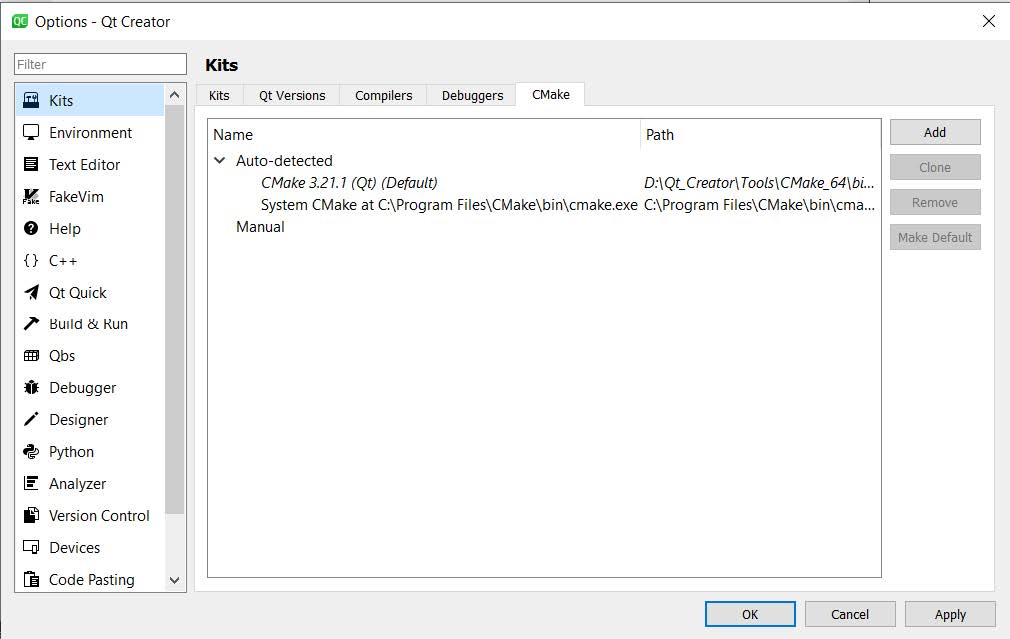
\includegraphics[width=0.6\textwidth]{content/1/chapter2/images/48.jpg}\\
图2.48 Qt Creator CMake路径设置
\end{center}

虽然缺少手工定义,但Qt Creator能够发现系统中的CMake安装。自动检测部分下的第一个是与Qt Creator一起提供的CMake可执行文件,第二个是系统的CMake安装。要选择在Qt Creator中运行的CMake可执行文件,请选择所需的条目并单击Make Default按钮。

添加一个新的CMake可执行文件,单击add。这将在Manual部分添加一个新条目,并弹出一个窗口来填写新条目的详细信息。

\begin{center}
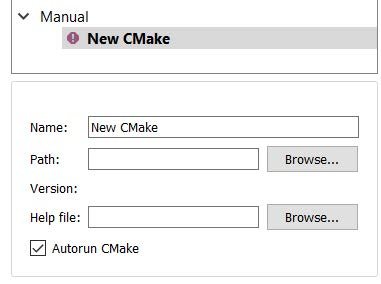
\includegraphics[width=0.4\textwidth]{content/1/chapter2/images/49.jpg}\\
图2.49 添加新的CMake可执行文件
\end{center}

窗口字段的详细描述如下:

\begin{itemize}
\item 
Name: 用于区分新的CMake可执行条目的唯一名称。

\item 
Path: CMake可执行路径(CMake/CMake.exe)。

\item 
Version: CMake的版本(由Qt Creator推导)。

\item 
Help file: 用于可执行文件的可选Qt Creator帮助文件,在按F1时出现CMake帮助。

\item 
Autorun CMake: 检查CMakeLists.txt文件的更改,以自动运行CMake。
\end{itemize}

填写详细信息后,单击Apply将新的CMake可执行文件添加到Qt Creator中。若打算使用Qt Creator,请不要忘记将其设置为默认值。

\hspace*{\fill} \\ %插入空行
\noindent
\textbf{创建CMake项目}

在Qt Creator中创建CMake项目的步骤,与创建常规项目的步骤完全相同。Qt Creator不将CMake视为外部构建系统生成器,它允许用户在三个构建系统生成器之间进行选择,分别是qmake、cmake和qbs。

要在Qt Creator中创建一个CMake项目,点击File | New File or project…(Ctrl + N),从新建文件或项目窗口选择项目类型。这里使用Qt Widgets Application作为我们的例子。

\begin{center}
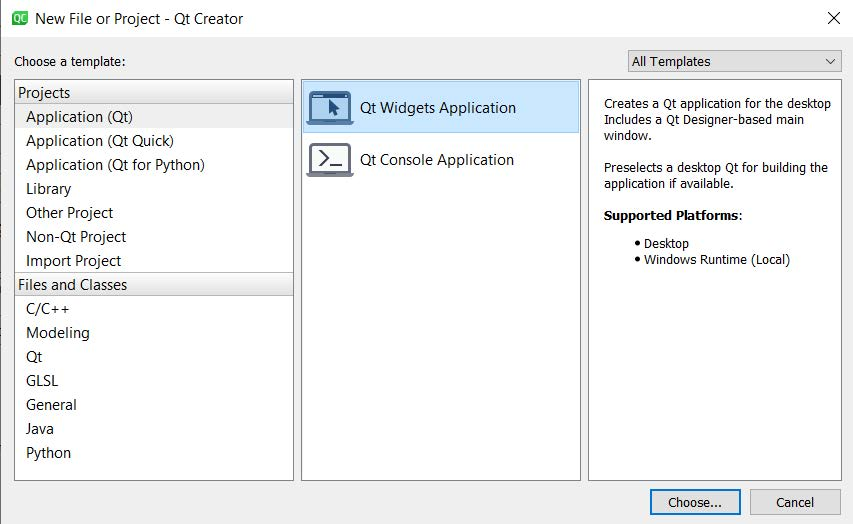
\includegraphics[width=0.6\textwidth]{content/1/chapter2/images/50.jpg}\\
图2.50  Qt Creator新建文件或项目窗口
\end{center}

选择之后,将出现项目创建向导。根据需要填写详细信息。在Define Build System步骤中选择CMake,如下图所示:

\begin{center}
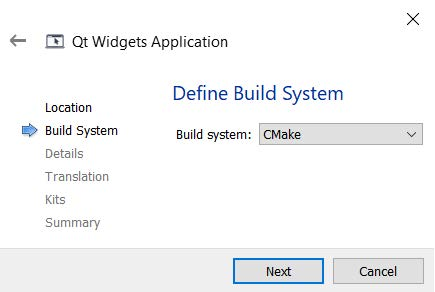
\includegraphics[width=0.4\textwidth]{content/1/chapter2/images/51.jpg}\\
图2.51  Qt Creator新建项目向导构建系统选择
\end{center}

这样就得到了一个带有CMake构建系统的Qt应用程序。

新建的CMake项目如下图所示:

\begin{center}
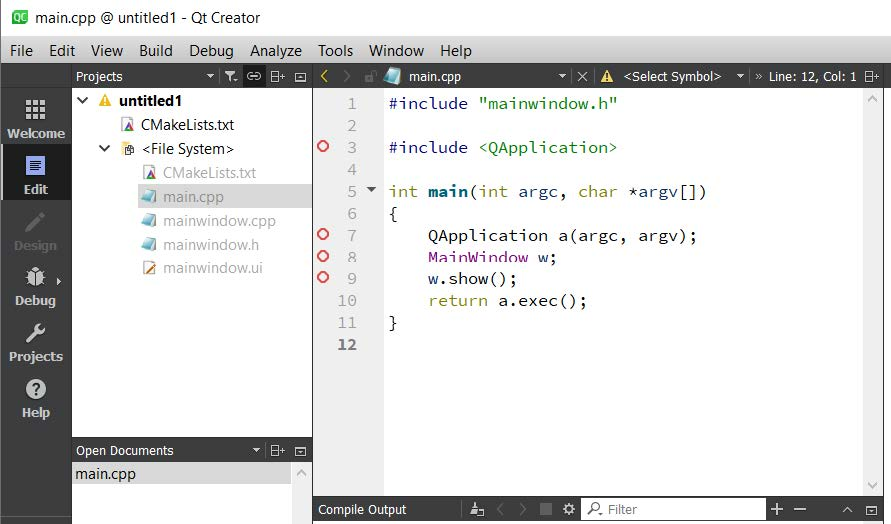
\includegraphics[width=0.6\textwidth]{content/1/chapter2/images/52.jpg}\\
图2.52 生成的基于CMake的Qt widgets应用项目
\end{center}

\hspace*{\fill} \\ %插入空行
\noindent
\textbf{打开现有的CMake项目}

Qt Creator中打开现有的CMake项目,通过File | Open File or Project... (Ctrl + O)(Ctrl + O)菜单项。选择项目的顶层CMakeLists.txt文件,然后单击Open。Qt Creator将提示,需要为项目选择一个工具包。选择相应套件,然后单击Configure Project按钮。将打开项目,CMake配置步骤将与所选套件一起运行。

例如,用Qt Creator打开的CMake最佳实践项目如下图所示:

\begin{center}
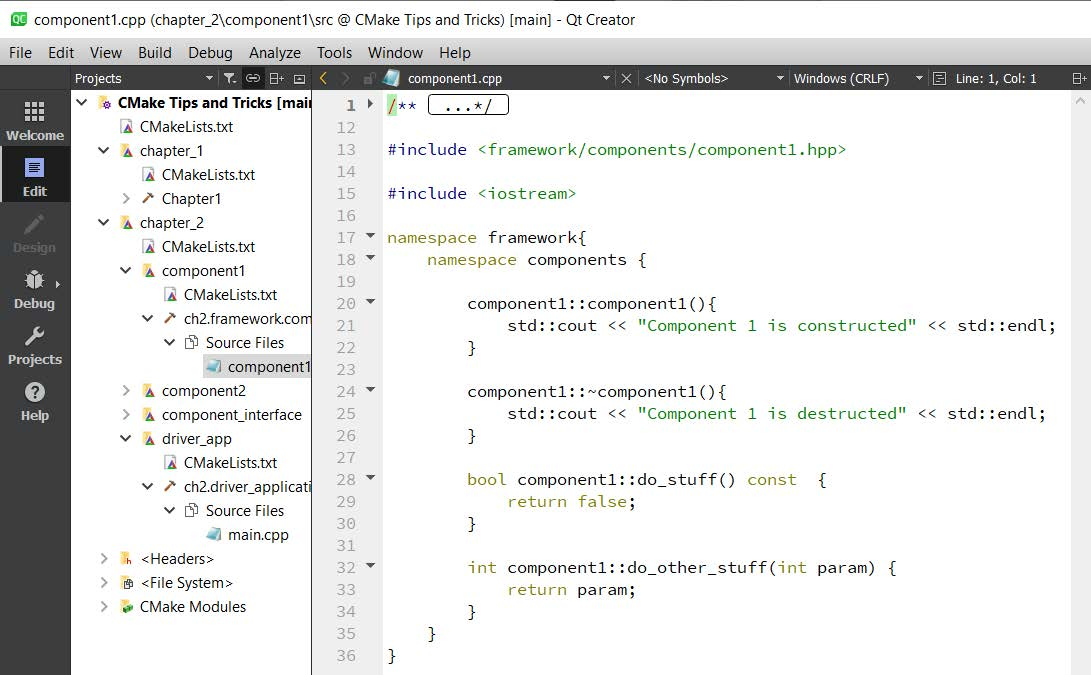
\includegraphics[width=0.8\textwidth]{content/1/chapter2/images/53.jpg}\\
图2.53 Qt Creator中查看CMake Tips and Tricks示例项目
\end{center}

第一次打开CMake项目后,Qt Creator会在项目的根目录下创建一个名为CMakeLists.txt.user的文件。该文件包含不能存储在CMakeLists.txt文件中的特定于Qt的详细信息,如工具包信息和编辑器设置。

\hspace*{\fill} \\ %插入空行
\noindent
\textbf{配置和构建}

大多数情况下(项目打开并保存更改到CMakeLists.txt),Qt Creator将自动运行CMake配置,无需手动运行。要手动运行CMake配置,请单击“Build | Run CMake”菜单项。

配置完成后,按左上角的锤子图标来构建项目。也可以使用快捷键“Ctrl + B”。这将构建整个CMake项目。要只构建特定的CMake目标,请使用“Build”按钮旁边的“Locator”。输入cm,然后按键盘上的空格键。

\begin{center}
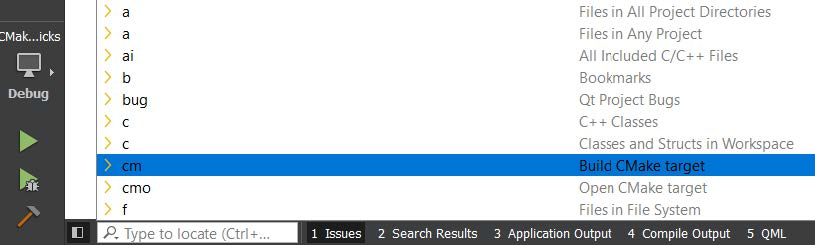
\includegraphics[width=0.8\textwidth]{content/1/chapter2/images/54.jpg}\\
图2.54 Qt Creator定位器建议
\end{center}

定位器将显示可用于构建的CMake目标。通过高亮显示并按下Enter键来选择所需的目标,或者直接使用鼠标单击目标。

\begin{center}
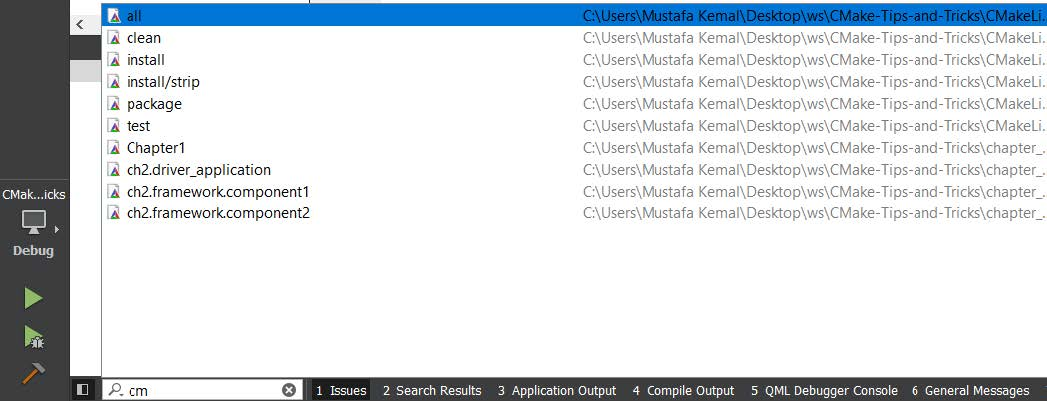
\includegraphics[width=0.8\textwidth]{content/1/chapter2/images/55.jpg}\\
图2.55 可构建的CMake目标显示在定位器上
\end{center}

将构建选中的CMake目标(当然还有其依赖项)。

\hspace*{\fill} \\ %插入空行
\noindent
\textbf{运行和调试}

要运行或调试CMake目标,请按下套件选择按钮(左侧导航栏上的计算机图标)并选择CMake目标。然后,单击运行按钮(工具箱选择器下的播放图标)进行运行,或者单击调试按钮(带有bug的播放图标)进行调试。

套件选择器菜单内容如下图所示:

\begin{center}
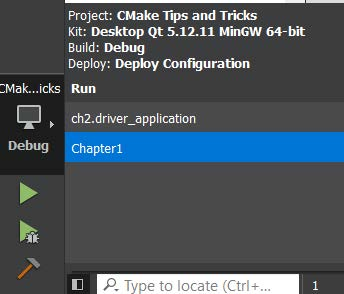
\includegraphics[width=0.5\textwidth]{content/1/chapter2/images/56.jpg}\\
图2.56 显示CMake目标的套件选择器
\end{center}

这里,我们总结了在Qt Creator中使用CMake的基础知识。要了解更高级的主题,可以参考扩展阅读中提供的资源。

















